\section{Redes neuronales}

\subsection{Introducci\'on}

Las redes neuronales se pueden definir  de distintas maneras:
\begin{itemize}
\item Como una forma de computación inspirada en modelos biológicos.
\item Como modelos matemáticos que se componen de un gran número de elementos procesables organizados en niveles, elementos de procesos muy interconectados que procesan información por medio de su estado dinámico como respuesta a entradas externas [  .
\item Modelos matemáticos para el procesamiento de información.
Redes interconectadas masivamente en paralelo de elementos simples (usualmente adaptativos) y con organización jerárquica, las cuales intentan interactuar con los objetos del mundo real del mismo modo que lo hace un sistema nervioso [Eduardo Caicedo].
\item Según Haykin(1994), una red neuronal es un procesador paralelo masivamente distribuido que tiene una facilidad natural para almacenar el conocimientos obtenido de la experiencia para luego hacerlos utilizable. 
\end{itemize}

\begin{figure}[H]
	\centering
	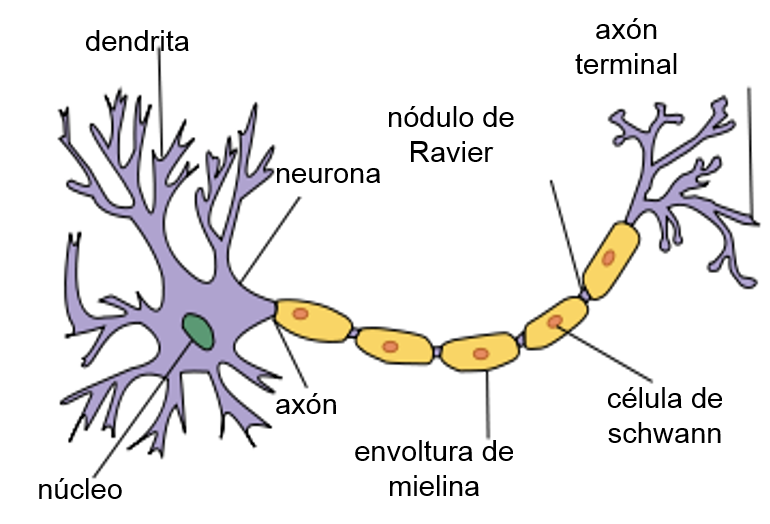
\includegraphics[width=10cm]{Capitulo2MarcoTeorico/Imagenes/red.png}	
	\caption{Red neuronal biologica.}
	\caption*{Tomado de \url{http://slideplayer.es/slide/92022/}.}
	\label{fig:redbiologica}	
\end{figure}
\subsection{Topologias de las redes neuronales}
la topologia o arquitectura de una red neuronal consiste de la organización y disposición de la neuronas en la red neuronal, la cual esta íntimamente ligada con el algoritmo (reglas) de aprendizaje utilizado, entre ellas tenemos.
\begin{itemize}
 \item \textbf{Redes monocapa:}
 En este tipo de red tenemos una capa de nodos de entrada desde el origen, que se proyecta en una capa de salida.
 \item \textbf{Redes multicapa:}
 la segunda clase de red neuronal se distingue por la presencia de una o mas capas ocultas, donde la neuronas son llamadas neuronas ocultas o unidades ocultas, siendo estas las que intervienen entre la entrada externa y la salida de la red de alguna manera útil.
 
\end{itemize}
\subsection{Mecanismos de aprendizaje}
 
\begin{itemize}
\item \textbf{Aprendizaje supervisado:}
Este tipo de aprendizaje es conocido así debido a que en el proceso de aprendizaje se realiza mediante un entrenamiento, controlado por un supervisor, quien define la salida para una entrada especifica.\\
\item \textbf{Aprendizaje no supervisado:} 
Este tipo de aprendizaje esta diseñado para aquellas redes neuronales que no requieren influencia externa, así que la red no recibe ninguna información por parte del entorno para decidir si la respuesta es la correcta o no.
\end{itemize}
\subsection{Algoritmo Backpropagation}

Algoritmos mas popular para el entrenamiento de redes neuronales, ya que muestra un desempeño optimo. 

\subsection{Normalización de datos}

Para que la red neuronal pueda calcular la salida se hace necesario tener datos numéricos, por lo tanto para aquellos datos que no lo son se hace necesario aplicar cierta técnicas de normalización donde se encuentre valores apropiados para representar las características simbólicas, ejemplo(  madrugada, mañana,tarde, noche).


